\clearpage
\section{Análisis bibliométrico de coocurrencia de palabras clave}
\label{sec:bibliometria}


\subsection{Estructura temática de la red}
\label{subsec:biblio-red}

La Figura~\ref{fig:red} presenta la visualización de red, en la que el tamaño
de cada nodo es proporcional a su frecuencia de aparición, la distancia entre
nodos refleja la intensidad de su coocurrencia y el color identifica el
agrupamiento asignado por el algoritmo de modularidad.

\begin{figure}[htbp]
    \centering
    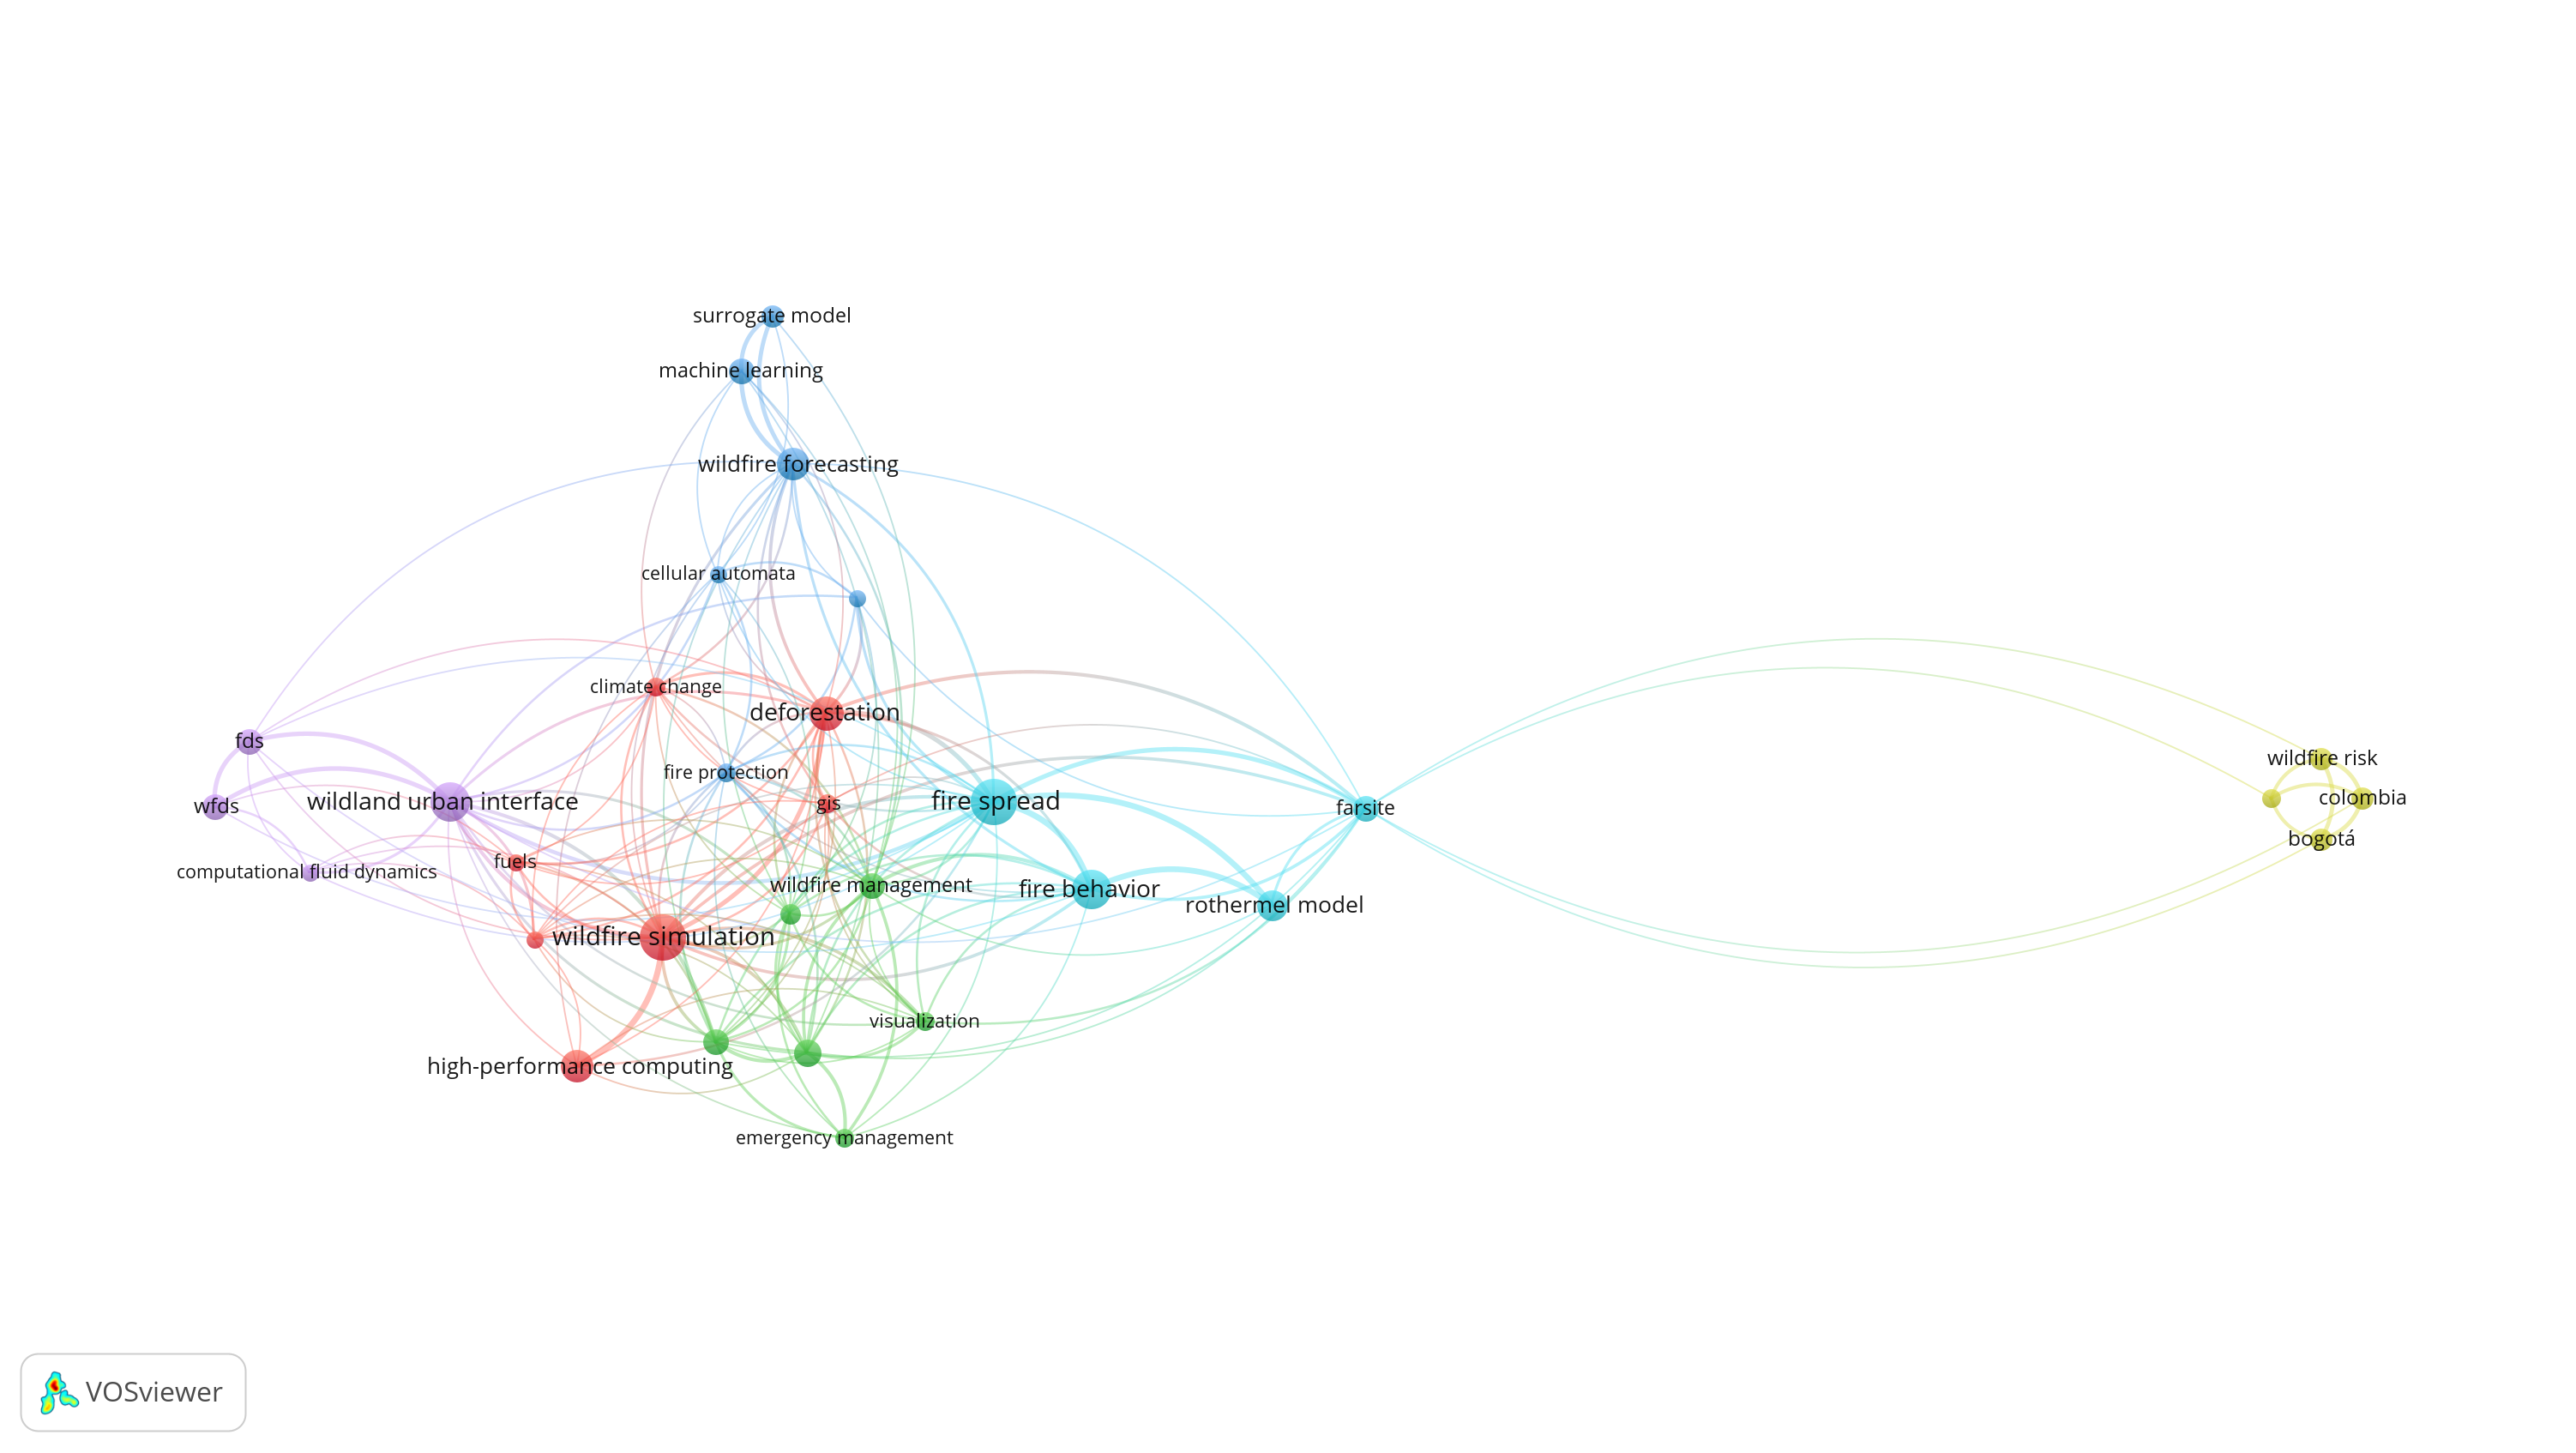
\includegraphics[width=0.95\textwidth]{Network}
    \caption{Red de coocurrencia de palabras clave del corpus revisado. El tamaño del nodo indica la frecuencia del término, la distancia entre nodos su intensidad de coocurrencia y el color el agrupamiento asignado. Elaboración propia con VOSviewer 1.6.21.}
    \label{fig:red}
\end{figure}

Los seis agrupamientos admiten la siguiente lectura temática:

\begin{description}
  \item[Simulación y modelado físico.] Articulado en torno a
  \emph{wildfire simulation}, incorpora \emph{cellular automata},
  \emph{fire spread model}, \emph{climate change}, \emph{fuels}, \emph{wind} y
  \emph{high-performance computing}. Constituye el núcleo metodológico de la
  red y ocupa una posición central.

  \item[Predicción y aprendizaje automático.] Reúne \emph{wildfire
  forecasting}, \emph{machine learning} y \emph{surrogate model} en la región
  superior del mapa. Su composición sugiere una línea orientada a la
  sustitución de simulaciones costosas por modelos aproximados.

  \item[Comportamiento del fuego.] Agrupa \emph{fire behavior},
  \emph{rothermel model}, \emph{fire spread} y \emph{farsite}. Corresponde al
  aparato conceptual y a las herramientas operativas heredadas de la
  literatura fundacional.

  \item[Interfaz urbano-forestal.] Compuesto por \emph{wildland urban
  interface}, \emph{fds}, \emph{wfds} y \emph{computational fluid dynamics}.
  Su coherencia interna es alta, dado que FDS y su extensión WFDS son
  precisamente los modelos de dinámica de fluidos aplicados a este contexto.

  \item[Soporte a la decisión y gestión operativa.] Integra \emph{decision
  support systems}, \emph{decision making}, \emph{emergency management},
  \emph{wildfire management} y \emph{visualization}, orientado a la
  traducción de resultados de simulación en instrumentos de gestión.

  \item[Contexto de aplicación local.] Formado por \emph{bogotá},
  \emph{colombia}, \emph{cerros orientales} y \emph{wildfire risk}.
\end{description}

Este último agrupamiento ocupa una posición marcadamente periférica y se
conecta con el resto de la red casi exclusivamente a través de \emph{farsite}.
Conviene subrayar que dicha separación no debe interpretarse como evidencia de
una línea de investigación autónoma: refleja el reducido número de documentos
de contexto local incorporados al corpus y el escaso solapamiento de su
vocabulario con el del resto de la literatura.

\subsection{Evolución temporal}
\label{subsec:biblio-overlay}

La Figura~\ref{fig:overlay} reproduce la misma red coloreada según el año
medio de publicación de los documentos en que aparece cada término.

\begin{figure}[htbp]
    \centering
    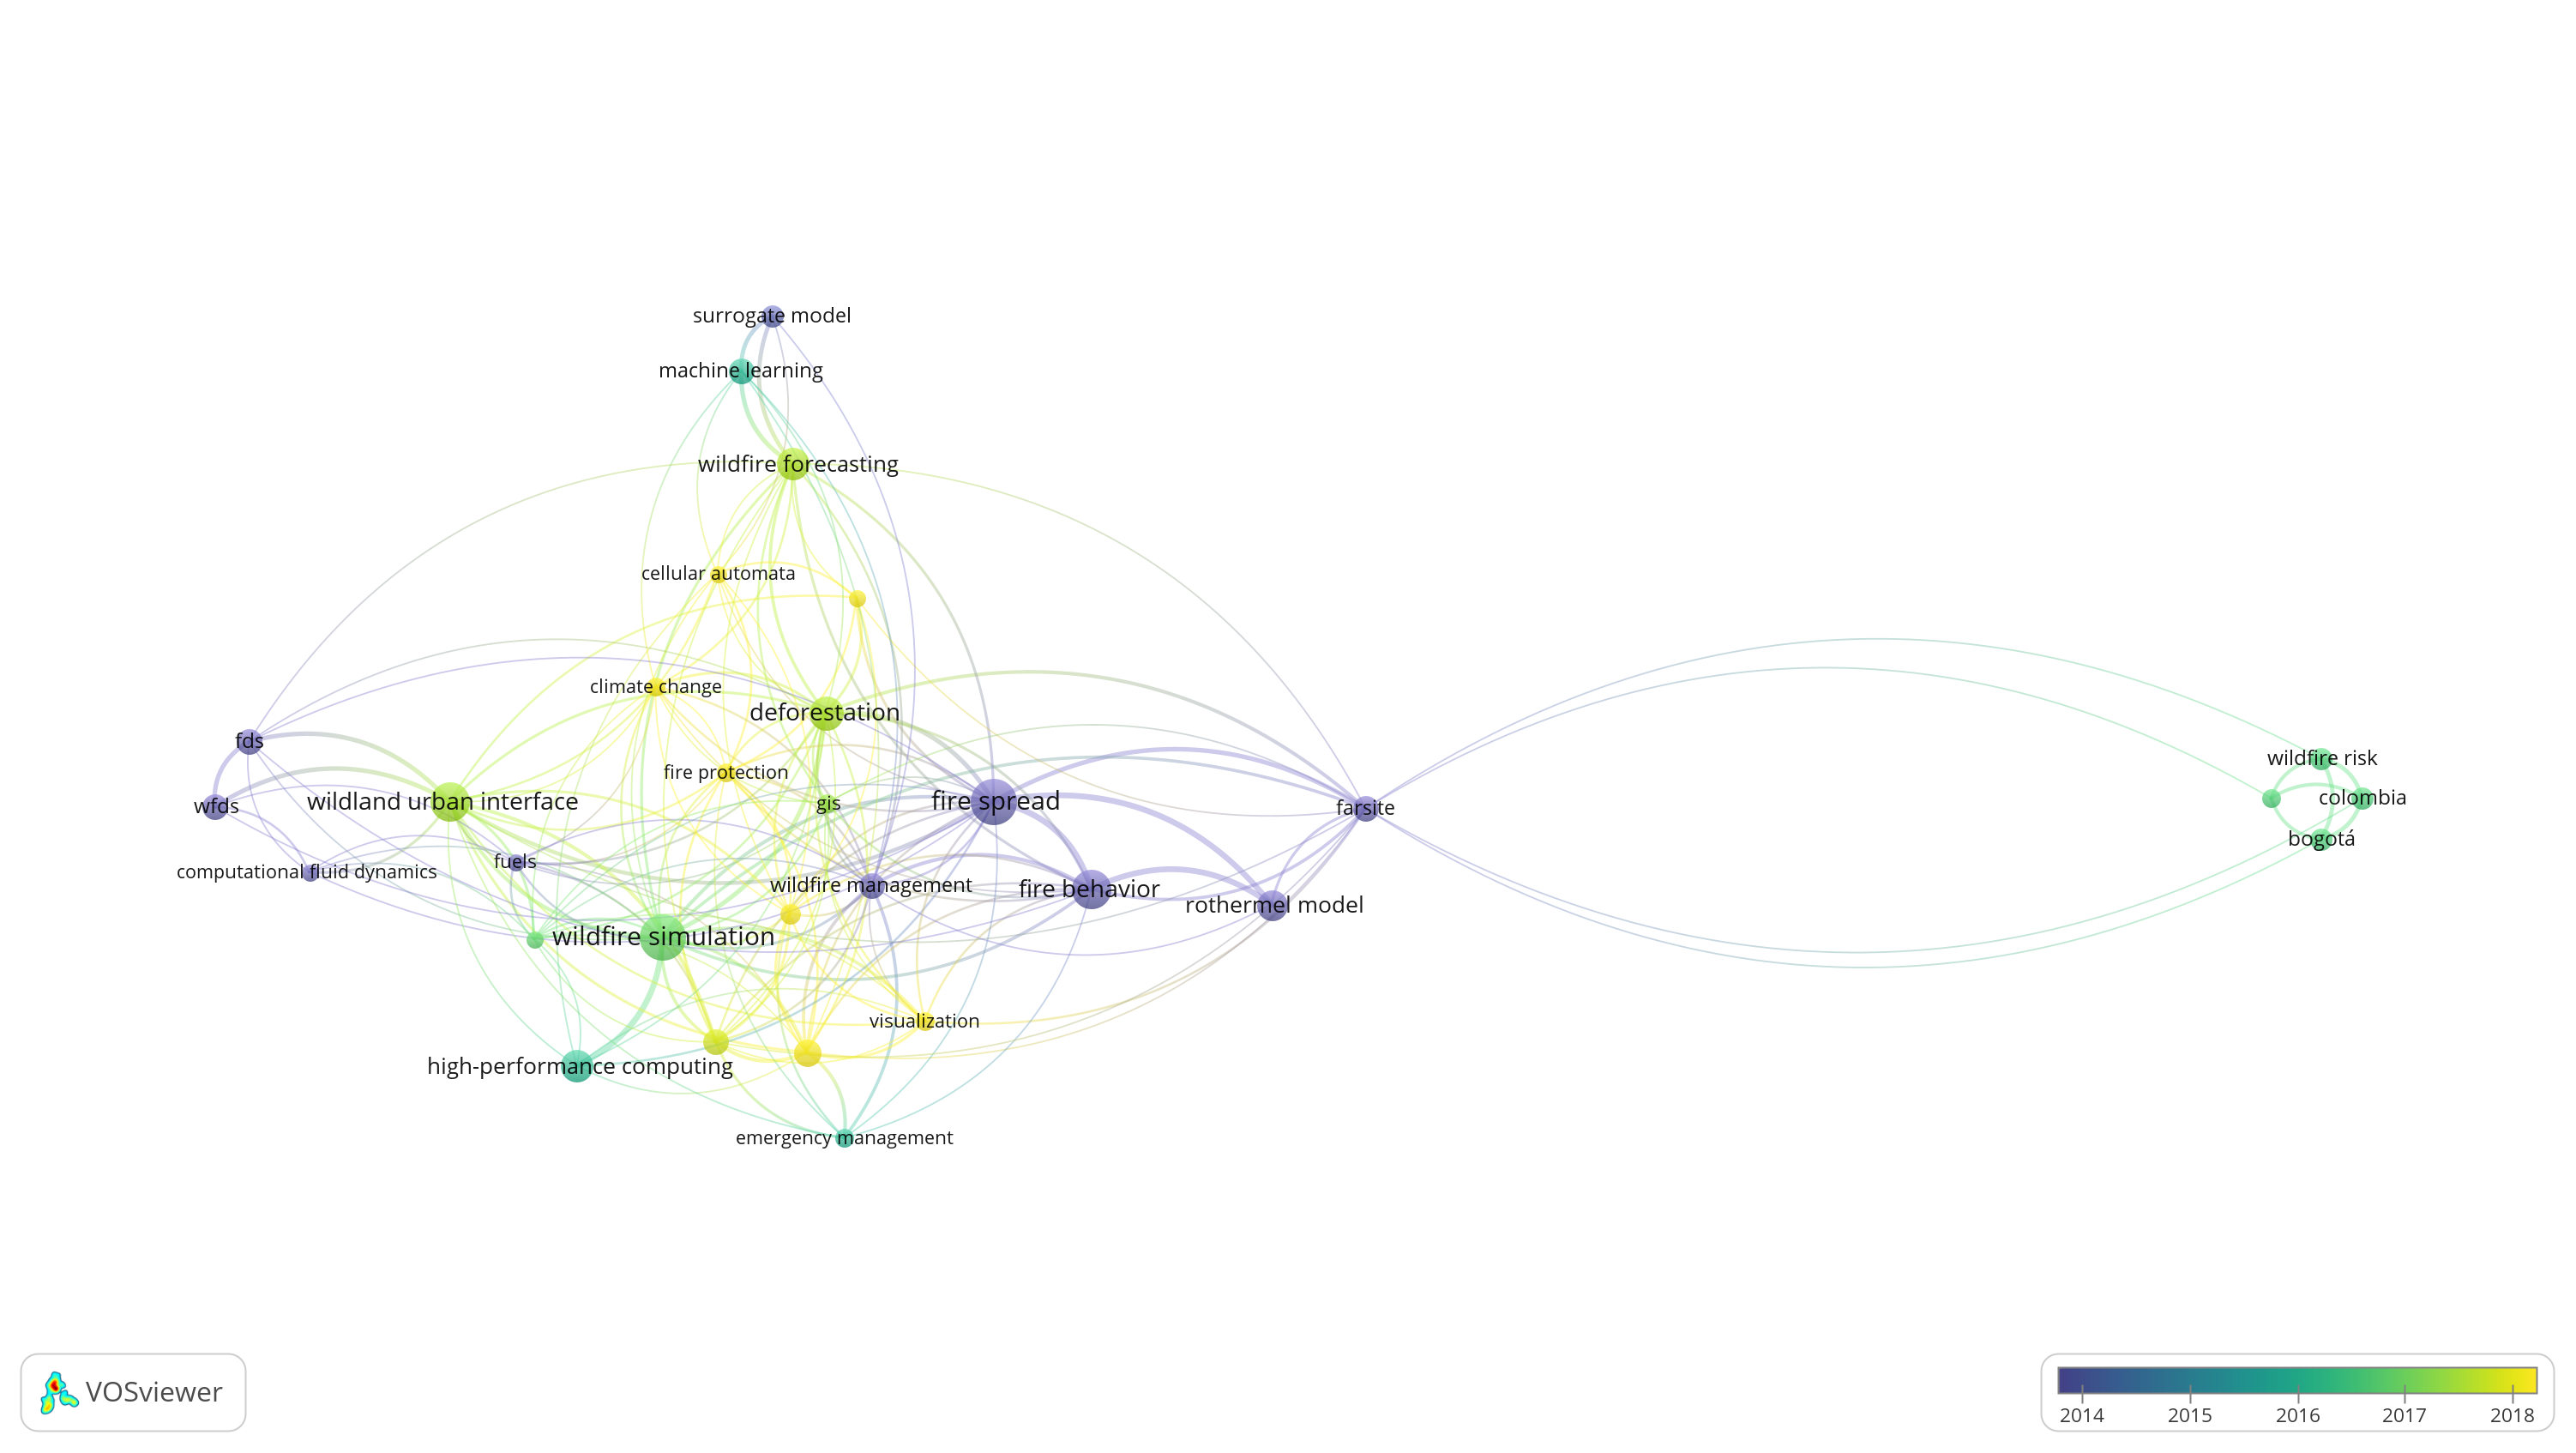
\includegraphics[width=0.95\textwidth]{overlay}
    \caption{Superposición temporal de la red de coocurrencia. Los nodos se colorean según el año medio de publicación de los documentos en que aparece cada término, en una escala que abarca de 2014 (violeta) a 2018 (amarillo). Elaboración propia con VOSviewer 1.6.21.}
    \label{fig:overlay}
\end{figure}

El extremo antiguo de la escala corresponde a \emph{fire behavior},
\emph{rothermel model}, \emph{farsite}, \emph{fire spread}, \emph{fds} y
\emph{wfds}: el conjunto de modelos físicos y herramientas consolidadas que
opera como sustrato del campo. En posiciones intermedias se sitúan
\emph{wildfire simulation}, \emph{high-performance computing},
\emph{wildland urban interface}, \emph{machine learning} y \emph{surrogate
model}. Los valores más recientes se concentran en \emph{decision support
systems}, \emph{decision making}, \emph{visualization}, \emph{gis},
\emph{fire protection} y \emph{cellular automata}.

El patrón sugiere un desplazamiento del interés desde la formulación de
modelos de comportamiento del fuego hacia su integración en sistemas de
soporte a la decisión y su comunicación mediante herramientas geoespaciales y
de visualización. Es decir, el énfasis parece haberse trasladado de la
pregunta por cómo modelar la propagación hacia la pregunta por cómo hacer
operativo ese modelado.

Debe advertirse, no obstante, que la escala cromática comprende únicamente el
intervalo 2014--2018 pese a que el corpus abarca desde 1967. VOSviewer calcula
un promedio ponderado por término y recorta los extremos de la distribución,
de modo que los colores expresan posiciones relativas dentro del corpus y no
años de publicación en sentido estricto.

\subsection{Densidad de ítems}
\label{subsec:biblio-densidad}

La Figura~\ref{fig:densidad} muestra la visualización de densidad, en la que
la intensidad cromática resulta de la concentración de términos y de su peso
en cada región del plano.

\begin{figure}[htbp]
    \centering
    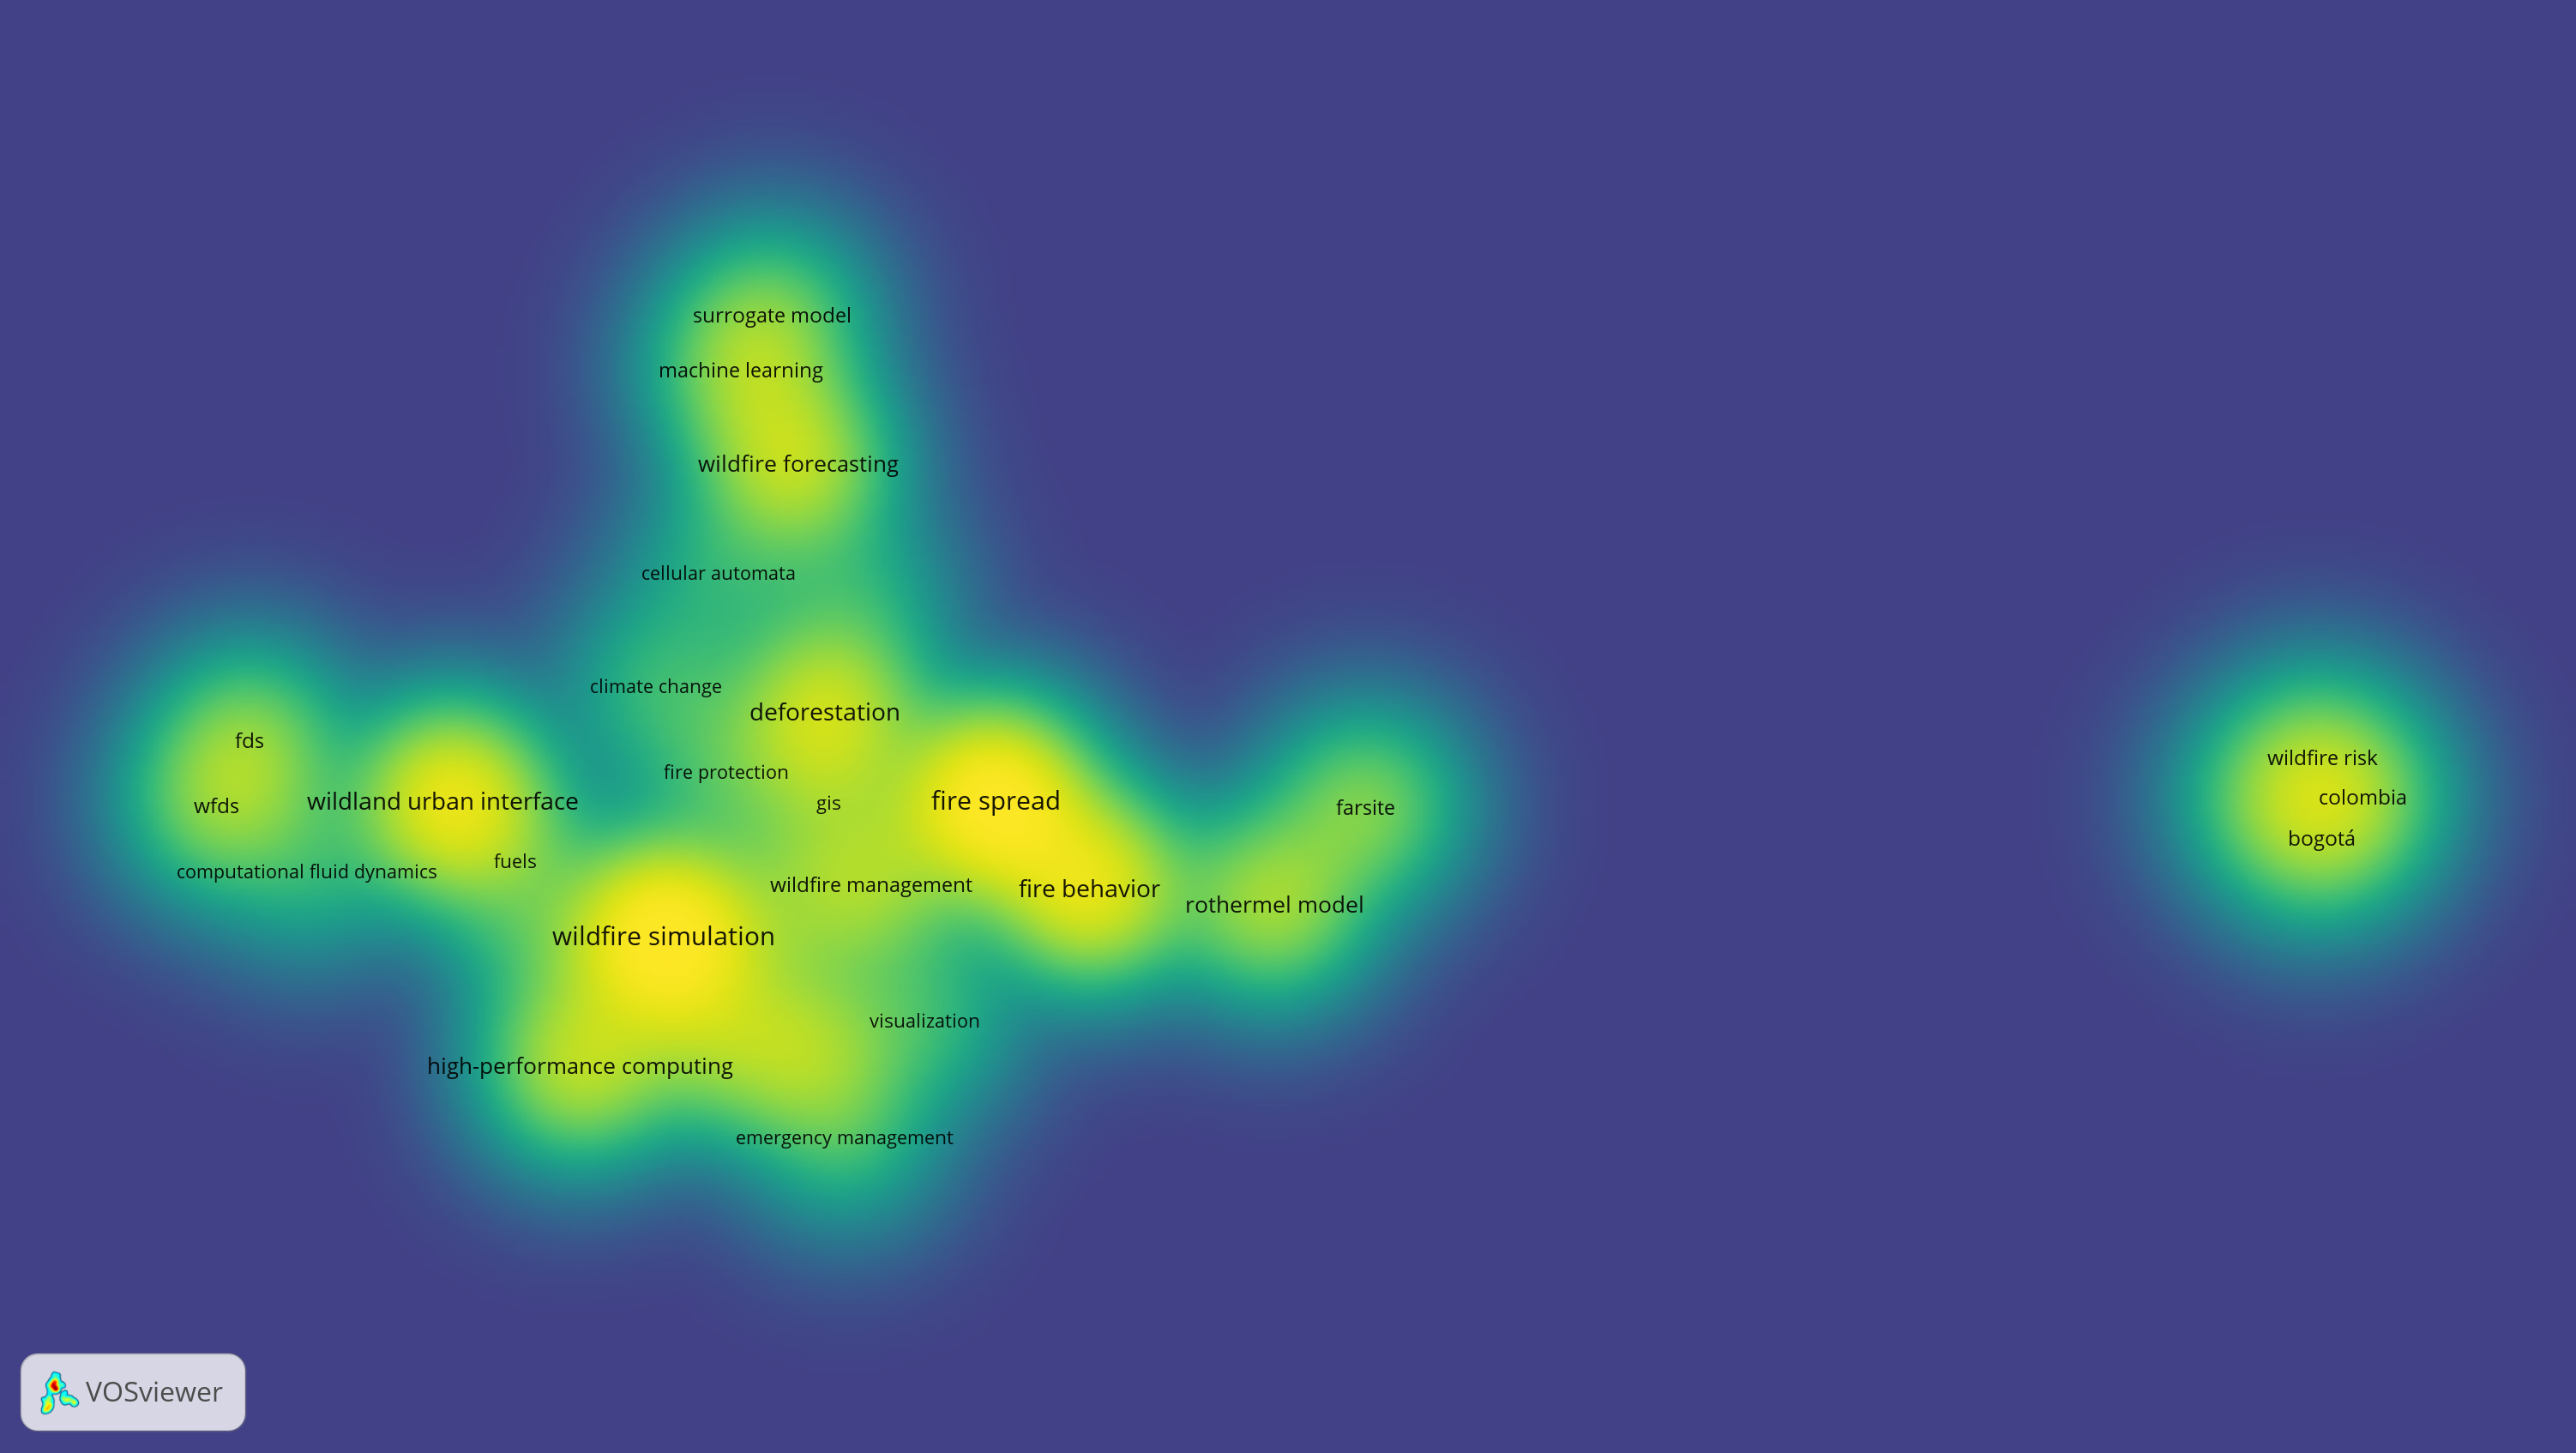
\includegraphics[width=0.95\textwidth]{Density}
    \caption{Visualización de densidad de la red de coocurrencia. La intensidad cromática resulta de la concentración de términos y de su peso en cada región del plano. Elaboración propia con VOSviewer 1.6.21.}
    \label{fig:densidad}
\end{figure}

Se distinguen cuatro concentraciones principales. La más extensa se organiza
alrededor de \emph{wildfire simulation}, \emph{high-performance computing} y
\emph{decision support systems}, y constituye el centro de gravedad temático
del corpus. Una segunda concentración, de intensidad comparable, agrupa
\emph{fire behavior}, \emph{fire spread} y \emph{rothermel model}. Las dos
restantes, de menor extensión, corresponden a \emph{machine learning} y
\emph{surrogate model} en la región superior, y a \emph{wildland urban
interface} en el flanco occidental.

El espacio comparativamente poco denso que media entre la concentración de
aprendizaje automático y la de soporte a la decisión resulta de interés: indica
que ambos conjuntos de términos rara vez concurren en un mismo documento. La
integración entre técnicas de aproximación por aprendizaje y sistemas
operativos de gestión aparece, en consecuencia, como un espacio escasamente
transitado en la literatura revisada.

